\documentclass[11pt]{article}
\usepackage{geometry}
\usepackage[onehalfspacing]{setspace}
\usepackage{fancyhdr}
\usepackage{lastpage}
\usepackage{microtype}
\usepackage{hyperref}
\usepackage{xurl}
\hypersetup{
    colorlinks=true,
    linkcolor=black,
    citecolor=blue,
    bookmarksopen=true,
    pdftitle={12g Seminarfacharbeit},
    pdfpagemode=FullScreen,
    }
\geometry{a4paper}

\usepackage[utf8x]{inputenc}
\usepackage{amsmath}
\usepackage{chngcntr}
\usepackage{graphicx}
\usepackage[colorinlistoftodos]{todonotes}
\usepackage{enumitem}
\usepackage{listings}
\usepackage{filecontents}
\usepackage{verbatim}
\usepackage{eurosym}
\usepackage[export]{adjustbox}
\usepackage[nohyperlinks]{acronym}
\usepackage[pagewise, modulo]{lineno}

\usepackage{fancyhdr}
\pagestyle{fancy}
\fancyhf{}
\fancypagestyle{plain}{}
\renewcommand{\headrulewidth}{0pt}


\usepackage{fontspec}
\usepackage{float}
\setmainfont{Arial}

\begin{document}
\begin{titlepage}

    \newcommand{\HRule}{\rule{\linewidth}{0.5mm}}
    \centering
    \textsc{\LARGE Schiller-Gymnasium Hameln}\\[1.5cm] % Name of your university/college
    \textsc{\Large 12g Seminarfacharbeit}\\[0.5cm] % Major heading such as course name
    \textsc{\Large Mathematik/Physik}\\[0.5cm]
    
    %----------------------------------------------------------------------------------------
    %	TITLE SECTION
    %----------------------------------------------------------------------------------------
    
    \HRule{} \\[0.4cm]
    { \huge \bfseries Umsetzung einer Künstlichen Intelligenz
    \\zur Erkennung handgeschriebener Zahlen}\\[0.4cm] % Title of your document
    \HRule{} \\[1.5cm]
     
    %----------------------------------------------------------------------------------------
    %	AUTHOR SECTION
    %----------------------------------------------------------------------------------------
    
    \begin{minipage}{0.4\textwidth}
    \begin{flushleft} \large
    \emph{Autor:}\\
    Bui Anh Minh Leon Phan\\
    \end{flushleft}
    \end{minipage}
    \begin{minipage}{0.4\textwidth}
    \begin{flushright} \large
    \emph{Tutoren:} \\
    Hr. Fistler, Hr. Dr.\ Kajari\\
    \end{flushright}
    \end{minipage}\\[2cm]
    
    %----------------------------------------------------------------------------------------
    %	DATE SECTION
    %----------------------------------------------------------------------------------------
    
    {\large 27. Januar 2023}\\[2cm] % Date, change the \today to a set date if you want to be precise
    
    %----------------------------------------------------------------------------------------
    %	LOGO SECTION
    %----------------------------------------------------------------------------------------
    
    
\includegraphics[width=120pt, keepaspectratio]{images/sghm}\\[2cm]
     
    %----------------------------------------------------------------------------------------
    
    \vfill
    
    \end{titlepage}

\newgeometry{
    left=50mm,
    right=10mm,
    top=15mm,
    bottom=30mm,
    footskip=15mm
}
\numberwithin{equation}{section}

\renewcommand{\contentsname}{Inhaltsverzeichnis}
\renewcommand{\figurename}{Abbildung}
\tableofcontents
\newpage
\rfoot{Seite \thepage}


\section{Abbildungsverzeichnis}
- Seite 2 bis 3

\newpage


\section{Abkürzungsverzeichnis}

\begin{acronym}
\acro{KI}{Künstliche Intelligenz}
\acro{CNN}{Faltendes Neuronales Netzwerk}
\end{acronym}
\newpage

\renewcommand\linenumberfont{\normalfont\small}
\setlength\linenumbersep{1cm}
\linenumbers{}

\section{Einleitung}
(Seite 5)
In der heutigen Zeit spielt Künstliche Intelligenz (KI) eine sehr wichtige Rolle in unserer
Gesellschaft.\label{1} Es gibt viele Anwendungsbereiche für KI, 
sei es im Bereich Verkehr, Gesundheit, Werbung oder auch Cybersicherheit.~\cite{useofki}
KI wird zum unverzichtbaren Mittel der Zukunft. So muss der
Forschungsstand zum Bereich KI besonders weit sein, da die Fehlerberechnungen auf das
Minimum beschränkt werden müssen.\label{2} Nun ist es aber so, dass die jetzigen KIs nur auf einzelne
Themen spezialisiert werden. Eine KI, die in mehreren Themengebieten
professionell funktionieren kann, ist heutzutage noch nicht möglich.~\cite{weakki}
Außerdem hinterfragt keiner, wie eine KI aufgebaut ist und wie dieser funktioniert.
Zum Schluss schreiben


\section{Künstliche Intelligenz}
Der Begriff Künstliche Intelligenz (KI) ist sehr schwer definierbar, denn es mangelt an der Defintion des Begriffs Intelligenz.
Allgemein kann die KI definiert werden als der Versuch, bestimmte Entscheidungsstrukturen von Menschen nachzubilden mithilfe von
Algorithmen. Manche Experten behaupten aber auch, dass eine KI nicht gleich eine KI ist, sondern sie in zwei Bereiche unterteilt werden kann.
Dabei wird die KI zwsichen einer starke KI und einer schwache KI unterschieden. Schwache KIs sind nur in bestimmten Teilbereichen in der Lage
an die menschliche Intelligenz heranzukommen. Doch sie ist nicht anpassungsfähig. Das bedeutet, dass eine schwache KI, die zum Beispiel auf Schach
spezialisiert wird, nur die Intelligenz im Bereich Schach besitzt. Selbstständiges fahren ist mit der KI nicht möglich. Dafür muss eine
andere KI spezialisiert werden, damit sie selbstständig fahren kann. Dagegen kann eine starke KI sich an derzeitigen Situatinen anpassen. Diese nennen sich auch ,,Superintelligenz''.
Solche starke KIs sind heutzutage noch nicht umsetzbar und es wird immer noch daran geforscht.
Die schwache KI, die in der Facharbeit speziell zur Erkennung von handgeschriebenen Zahlen programmiert wird, können in 2 Teilbereichen
unterteilt werden.
\begin{figure}[h]
\centering
\includegraphics[width=300pt, keepaspectratio]{images/ki\_kategorie}
\caption{Unterkategorien der Künstliche Intelligenz.}
\end{figure}
Eine Unterkategorie der KI wäre der Bereich Maschinelles Lernen. Maschinelles Lernen versucht mithilfe von Algorithmen mit einer großen Anzahl von
Daten ein Muster zu erkennen. Dazu werden die aus Daten gewonnen Erkenntnisse für Problemlösung verwendet oder der Algorithmus wird auf
die Daten zugeschnitten und verallgemeinert.
Der zweite Teilbereich wäre mehrschichtiges Lernen, das sehr an maschinelles Lernen ähnelt. Der Unterschied liegt aber an der Art und Weise, wie
sie mit den Daten arbeitet. Mehrschichtiges Lernen versucht das menschliche Gehirn zu imitieren durch ein künstliches Neuronales Netzwerk.
Durch das Imitieren sind die Strukturen vom mehrschichtigen Lernen deutlich komplexer als die vom maschinellen Lernen. Deswegen sind
sehr große Datensätzen von Vorteil für mehrschichtiges Lernen, da deutlich mehr Merkmale der Daten erkannt werden. Darauf basiert sich die KI
in der Facharbeit.
\subsection{Überwachtes Lernen}
Überwachtes Lernen ist eine Methode, wie die KI mit Daten lernen kann. Dazu hat die Datei 2 wichtige Merkmale, nämlich die Eingabe und die
Ausgabe. Die Eingabe wird an die KI zum Lernen geschickt und dabei gibt die KI ein Ergebnis aus. Mit der Ausgabe der Datei wird nun überprüft, ob
die Antwort, die die KI ausgegeben hat, übereinstimmt.
\begin{figure}[h]
    \centering
    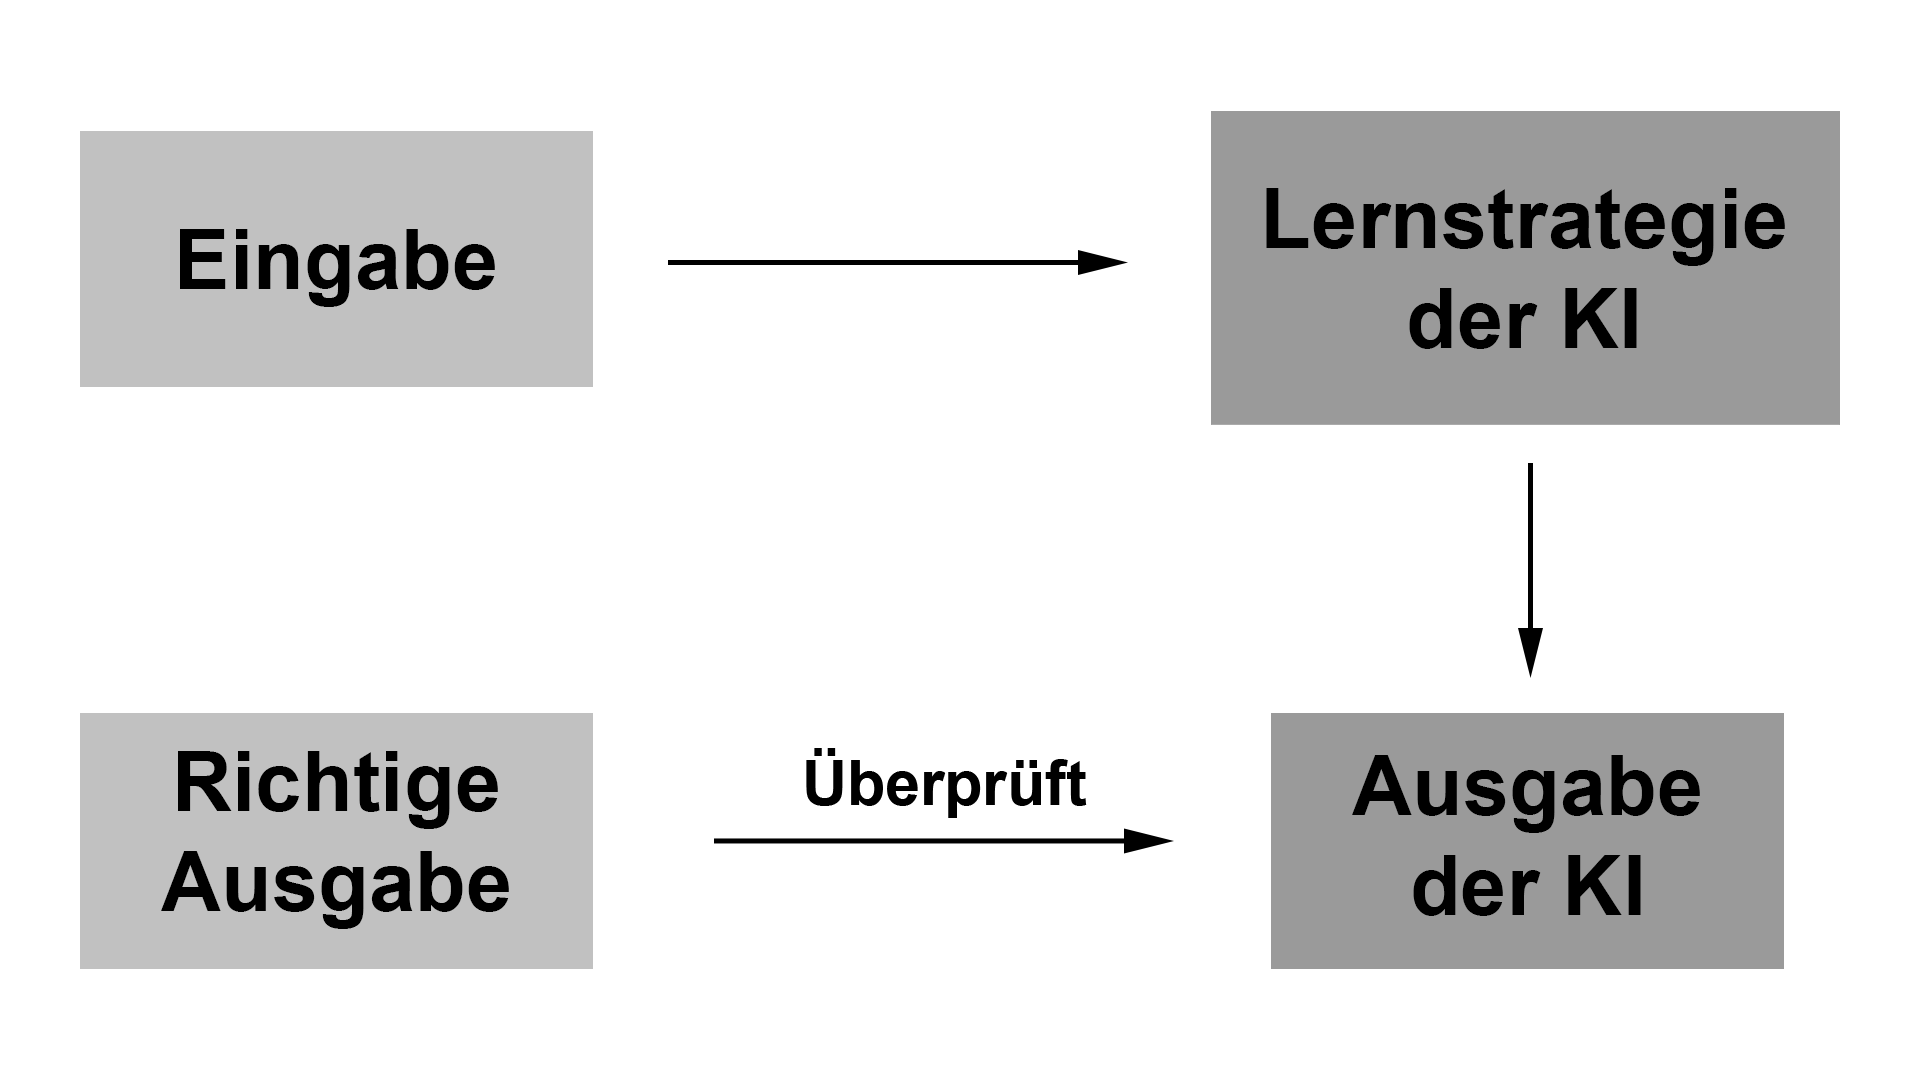
\includegraphics[width=300pt, keepaspectratio]{images/slearning}
    \caption{Ablauf eines überwachtes Lernen.}
\end{figure}
Falls sie nicht übereinstimmt, lernt die KI aus den Fehlern und verbessert sich
dadurch. Überwachtes Lernen ist eine angemessene Methode für das Problem der Facharbeit, da die Antwort, die die KI ausgibt, übereinstimmen muss.
Dadurch wird die Fehlerquote der KI möglichst kleingehalten, sodass eine genaue Erkennung der handgeschrieben Zahlen gelingen kann.
Dabei ist anzumerken, dass die KI zwei Arten von Lösungen angeben kann. In dem Fall wird die sogenannte Klassifikation als Lösungsart aktzeptiert.
Jede Zahl wird als eine eigene Klasse zugeordnet. Die KI gibt aus, um welche Klasse es sich handelt.

\section{Voraussetzung für mehrschichtiges Lernen}

Irgendetwas schreiben für die Voraussetzung

\subsection{Datensatz}
Datensätze sind für die KIs das wichtigste Werkzeug für das Lernen. Denn die Qualität des Datensatzen bestimmt die Lerneffizienz der KI.
Je schlechter die Qualität ist, desto schlechter lernt auch die KI. Wichtige Merkmale für Qualität ist die Auflösung, die Anzahl der Daten und die Varibialität.
Für mehrschichtiges Lernen wird ein großer Datensatz gebraucht. Dabei wird für die Problemlösung der MNIST Datensatz von Yann LeCun gewählt.
Sie besitzt insgesamt 70000 Bilder mit handgeschrieben Zahlen, die die Werte zwischen 0 und 9 besitzt. Jedes Bild hat ein 28$\times$28 Pixel
Format und ist farblos. Sie wird nur mit der Hellgikeit dargstellt zwischen 0 und 255. Außerdem hat jedes Bild einen Wert, um welche Zahl
es sich handelt, damit später geprüft werden kann, ob die KI die Zahl richtig erkannt hat oder ob sie falsch liegt.
\begin{figure}[h]
    \centering
    
\includegraphics[width=300pt, keepaspectratio]{images/number}
    \caption{Handgeschriebene Zahl als Abbildung in 28\times28 Pixeln dargestellt, dabei ist die richtige Ausgabe die Zahl 5.}
\end{figure}
Der Datensatz ist gut zum Lernen, denn sie besitzt keine Fehlwerte oder verzerrende Bilder, die die KI beim Lernen stören kann. Auch ist die
Auflösung in Ordnung und 70000 Bilder sind für kleine Aufgaben angemessen.

\subsection{Künstliches neuronales Netzwerk}
Im menschlichen Gehirn befinden sich großen Mengen von Neuronen, die miteinander interagieren. Dabei werden elektrische Signale an einzelne Neuronen
gesendet. Nun kann das einzelne Neuron entscheiden, ob sie dieses elektische Signal, was sie bekommen hat, weiterleitet zu den anderen Neuronen
oder sie das Signal ignoriert. In der Informatik kann dies umgeschrieben werden, ob das Neuron eine 0 oder eine 1 sendet, wobei die 1 als weitergeleitet gilt.
Da das menschliche Gehirn imitiert werden soll, werden künstliche Neuronen erschaffen, die einen Wert von den vorherigen künstlichen Neuronen verarbeitet wurden.
Durch die ganzen Verbindungen zwischen den Neuronen wird das auch als Netzwerk bezeichnet.
\begin{figure}[h]
    \centering
    \includegraphics[width=300pt, keepaspectratio]{images/neural\_network}
    \caption{Künstliches Neuronales Netz mit insgesamt 37 künstliche Neuronen in 6 Schichten verteilt.}
\end{figure}
Das Netzwerk kann unterschiedliche Anordnungen von künstlichen Neuronen besitzen. Die geeignetste Anordnung nennt sich das
konvolutionales neuronales Netzwerk (CNN), denn sie wird häufig für Bildererkennung verwendet. Grund dafür ist die Extrahierung der Merkmale
des Bildes. Denn bevor das Bild an die künstlichen Neuronen weitergeleitet werden, werden unnötige Merkmale mithilfe von Konvolution aus dem Bild entfernt, sodass der
Lernprozess der KI auf das Wichtigste begrenzt wird.

\section{Konvolutionales neuronales Netzwerk}

Das CNN kann in zwei Bereichen gegliedert werden. Der erste Bereich nennt sich
Merkmalsextraktion und ist dafür zuständig, die wichtige Merkmale des Bildes herauszufiltern. Im zweiten Bereich werden die
wichtigen Merkmalen aus der Merkmalsextraktion in die sogenannte Klassifikationsebene weitergeleitet. Dort fängt der Lernprozess
der KI an, die dann am Ende des Netzwerkes eine Klasse ausgibt.

\subsection{Klassifikationsebene}
In der Klassifikationsebene befindet sich das künstliches neuronales Netzwerk, die eine ähnliche Struktur wie bei Abbildung 4 hat.
Diese Struktur nennt sich auch Fully Connected Neural Network und ist in mehreren Schichten aufgebaut. In Abbildung 4 wäre die Anzahl
der Schichten $A = 6$. Die erste Schicht nennt sich Eingabeschicht, denn von dort kommen die Daten in die Neuronen rein, während bei
der letzte Schicht die KI ein Ergebnis ausgibt. Diese Schicht heißt Ausgabeschicht. Die Schichten dazwischen werden ausgeblendete Schicht genannt.
Die ausgeblendete Schichten sind wichtige Teile des Netzwerkes, denn durch diese werden Merkmale gesucht und analysiert. Das gibt nochmal
eine deutlich stärkere Lerntiefe für die KI.\@ Die einzelne Neuronen können einen Wert besitzen, sie wird als $ x_{i}^{(\alpha)} $ definiert,
wobei $ \alpha \in \{1,\ldots,A\} $ gilt. Der Index $i$ beschreibt um welches Neuron in der Schicht $\alpha$ es sich handelt. Dieser Wert
lässt sich aus den ganzen Verbindungen der vorherigen Schicht berechnen, indem sie wie in Abbildung 5 addiert werden. Dabei werden
die einzelne Werte $ x_{i}^{(\alpha-1)} $ mit einem Gewicht $ w_{i,j}^{(\alpha)} $ multipliziert, womit $ j \in \{1,\ldots,N_{\alpha-1}\} $ gilt.
$ N_{\alpha} $ beschreibt die Anzahl der Neuronen auf der Schicht $\alpha$. Allgemein gilt dann für die Berechnung
\begin{equation}
    x_{i}^{'(\alpha)} := (\sum_{j=1}^{N_{\alpha}} w_{i,j}^{(\alpha)} x_{j}^{(\alpha-1)}) + b_{i}^{(\alpha)} \quad i \in \{1,\ldots,N_{\alpha}\}, j \in \{1,\ldots,N_{\alpha-1}\}.
\end{equation}
Das $ b_{i}^{(\alpha)} $ in der Gleichung steht für Bias und ist ein weiterer Parameter zum Einstellen wie das Gewicht. Beide spielen hier eine wichtige Rolle
für das Weiterleiten der Neuronen. Das Gewicht entscheidet, wie wichtig der Wert vom Neuron ist. Je höher der Wert ist, desto entscheidener
ist das Neuron. Der Bias stellt ein, wie leicht das Neuron sich aktiviert. Auch hier gilt, je größer der Wert, desto entscheidener ist das Neuron.
Wichtig ist anzumerken, dass die Gewichte und die Biases verstellbare Parameter sind, die für das Lernen der KI eine wichtige Rolle
spielt. Eine weitere Sache, die hinzugefügt werden muss ist die Aktivierungsfunktion, denn sie gibt das Netzwerk eine Komplexität.
Ohne diese Komplexität wäre das Netzwerk linear, was Nachteile mit sich bringt für die KI. In Abbildung 6 ist die Regression bei einer
nicht lineare Struktur deutlich besser als dies einer lineare Struktur. Welche Aktivierungsfunktionen verwendet werden kommt in Lektion AKTIVIERUNGSFUNKTION
dran. So ergibt sich
\begin{equation}
    x_{i}^{(\alpha)} := f^{(\alpha)}(x_{i}^{'(\alpha)}) = f^{(\alpha)}((\sum_{j=1}^{N_{\alpha}} w_{i,j}^{(\alpha)} x_{j}^{(\alpha-1)}) + b_{i}^{(\alpha)}).
\end{equation}
Nun kann die Schicht auch als einen Vektor angesehen werden, wobei die Neuronen die Elemente vom Vektor sind. Folglich kann das Netzwerk
in Abbildung 4 in einem Matrixblock umgeschrieben werden. So definiert sich
\begin{equation}
    \vec{x}^{(\alpha)} := \begin{bmatrix}x_{1}^{(\alpha)} \\ x_{2    }^{(\alpha)} \\ \ldots \\ x_{N_{\alpha}}^{(\alpha)} \end{bmatrix}.
\end{equation}



\subsubsection{Aktivierungsfunktion}
- Seite 9
- Berechnet die Abweichungen der Genauigkeit des neuronalen Netzwerkes mit der Verlustfunktion
- Je kleiner der Wert, desto besser

\subsection{Feature Extraction??/Merkmalsextraktion (DeepL)}
Die Merkmalsextraktion besteht aus mehreren Schichten von Operationen mit dem das eingebene Bild verarbeitet wird.
Eine Hauptoperation ist der 2D Konvolution, denn diese Operation ist dafür zuständig, dass wichtige Merkmale gefiltert werden.
Weitere wichtige Operationen ist der Max-Pooling und der Flattening. Aufgabe von Max-Pooling ist es unnötige Merkmale
zu ignorieren, indem nur die hellsten Pixel rausgefiltert werden. Die Dimension des Bildes halbiert sich. Flattening ist für die Übertragung auf die Klassifikationseben zuständig,
indem die Matrix des Bildes in einen Vektor geflacht wird, sodass die KI optimal lernen kann.
ABBILDUNG (FEATURE EXTRACTION, HIER KÖNNEN WIR JA SCHONMAL ANFANGEN UNSERE KI ZU BAUEN)
Das Bild kann in einer 28\times28 Matrix dargestellt werden
\begin{equation}
    X^{(1,1)} := (x_{ij}) \quad i \in \{1,\ldots,28\}, j \in \{1,\ldots,28\}.
\end{equation}
Der erste Index beschreibt auf welcher Schicht die Variable sich befindet und der zweite Index beschreibt auf welches
Bild sie drauf bezieht, denn in einer Schicht können mehrere Bilder vorkommen. Dies nennt sich Tiefe. Da am Anfang aber nur ein Bild eingegeben wird, gilt
$B^{(1)} = 1$. Für die nächsten Schichten gilt im Allgemeinen
\begin{equation}
    X^{(\alpha,\beta)} := (x_{ij}) \quad i \in \{1,\ldots,m_{x}^{(\alpha,\beta)}\}, j \in \{1,\ldots,n_{x}^{(\alpha,\beta)}\}.
\end{equation}
Die Werte $m_{x}^{(\alpha,\beta)}$ und $n_{x}^{(\alpha,\beta)}$ werden basiert auf die Operation berechnet, wobei
$\alpha \in \{1,\ldots,A\}$ und $\beta \in \{1,\ldots,B^{(\alpha)}\}$. Dabei ist die Anzahl der Tiefe von der jeweilige Schicht abhängig.


\subsubsection{2D Konvolution}
Mithilfe von 2D Konvolution können wichtige Merkmale herausgefiltert werden. Damit sie aber herausgefiltert werden kann, wird
eine neue Matrix definiert, die auch als Kernel genannt wird
\begin{equation}
    K^{(\alpha,\beta)}:=(k_{i,j})^{(\alpha,\beta)} \quad i \in\{1;2;\ldots;m_{k}^{(\alpha,\beta)}\}, j \in\{1;2;\ldots;n_{k}^{(\alpha,\beta)}\}
\end{equation}
Wenn der Kernel nach bestimmten Mustern definiert wurde, entsteht durch die 2D Konvolution eine neue Matrix, in dem Fall ein neues Bild
ABBILDUNG CONVOLUTION
Diese neue Matrix wird definiert als 
\begin{equation}
    A := (a_{i,j}) \quad i \in \{1,\ldots,m_{a}\}, j \in \{1,\ldots,n_{a}\},
\end{equation}
wobei $ m_a = m_x - m_k + 1 $ und $ n_a = n_x - n_k + 1 $
Da sowohl die Eingabe des Bildes, sowie der Kernel beide Matritzen sind, kann mit der 2D Konvolution gerechnet werden. Sie ist
folgendermaßen defininiert
\begin{equation}
    a_{i,j} = (X \ast K)_{i,j} := \sum_{m'=1}^{m_{k}} \sum_{n'=1}^{n_{k}} x_{i-m'+1,j-n'+1}k_{m',n'}. \label{Conv}
\end{equation}
Eine weitere Operation, die sehr wichtig für die 2D Konvolution ist der Cross Correlation
\begin{equation}
    a_{i,j} = (X \star K)_{i,j} := \sum_{m'=1}^{m_{k}} \sum_{n'=1}^{n_{k}} x_{i+m'-1,j+n'-1}k_{m',n'}.
\end{equation}
Aus~\eqref{Conv} wird deutlich, dass Cross Correlation nichts anderes ist als eine 2D Konvolution, wo nur der Kernel um 180$^{\circ}$
rotiert ist. Dies wird später für die Fehlerrückführung in Kapitel 6.4.1 wichtig sein. Wenn die Schichten und die Tiefen der
Merkmalsextraktion berücksichtigt werden, so gilt für die nächste Schicht
\begin{equation}
    x_{i,j}^{(\alpha,\beta)} = f^{(\alpha)}((\sum_{\beta'=1}^{B^{(\alpha-1)}} \sum_{m'=1}^{m_{k}} \sum_{n'=1}^{n_{k}} x_{i+m'-1,j+n'-1}^{(\alpha-1,\beta')}k_{m',n'}^{(\alpha,\beta')})+b_{i,j}^{(\alpha,\beta)})
\end{equation}


\subsubsection{Max-Pooling}

\subsubsection{Flattening??}
Damit die Ki mit der Matrix lernen kann, muss diese Matrix in einen Vektor umgewandelt werden
\begin{equation}
    \vec{x}^{(\alpha,\beta)} := vec_{n_{x}^{(\alpha,\beta)}, m_{x}^{(\alpha,\beta)}}(X^{(\alpha-1,\beta)T})
\end{equation}

\subsection{Verlustfunktion}

\subsection{Optimierung}
- Seite 10 bis 12
- Für die Optimierung benutzen wir die ADAM Optimierer
\subsubsection{Fehlerrückführung}
- Eine Methode, um die Gradiente für die Optimierung zu berechnen

\section{Umsetzung}

\subsection{Werkzeuge}
- Seite 14
- Python wird hier verwendet, da gut für Data Science
- Hierfür wird NumPy benutzt für Matrix
- Auch wird der Matplotlib verwendet für Visualisierungen

\subsection{Trainingsphase}
- Daten müssen in 3 Sets aufgeteilt werden: Training, Test und Validation
- Irgendwo muss noch Overfitting und Underfitting rein, das mit Validation vermieden wird

\subsection{Auswertung}
- Seite 14
- Verschiedene Grafiken werden ausgewertet
- Z.B. Lernverlauf
- Accuracy anschauen
- Wert der Verlustfunktion im Verlauf anschauen
\subsubsection{Trainingsdaten}
\subsubsection{Validationsdaten}
\subsubsection{Testdaten}


\section{Schlussfolgerung}
- Seite 19
Paar Formeln, wobei gilt:
Linare Funktion zwischen zwei Neuronenschichten:
\[ \vec{x}^{(\alpha)}=f^{(\alpha)}(W^{(\alpha)} \vec{x}^{(\alpha-1)} + \vec{b}^{(\alpha)}) \]
RelU:
\[ x_i^{(\alpha)} := f^{(\alpha)}(x_i^{'(\alpha)}) \]
\[ x_i^{(\alpha)}= \left\{
	\begin{array}{ll}
		x_i^{'(\alpha)}  & \mbox{falls } x_i^{'(\alpha)} > 0 \\
		0 & \mbox{falls } x_i^{'(\alpha)} \leq 0
	\end{array}
\right. \]
Ableitung von RelU:
\[ \frac{\partial x_i^{(\alpha)}}{\partial x_i^{'(\alpha)}} = \left\{
	\begin{array}{ll}
		1  & \mbox{falls } x_i^{'(\alpha)} > 0 \\
		0 & \mbox{falls } x_i^{'(\alpha)} \leq 0
	\end{array}
\right. \]
Softmax:
\[ x_i^{(\alpha)} = \frac{e^{x_i^{'(\alpha)}}}{\sum_{j=1}^{N_{\alpha}} e^{x_i^{'(\alpha)}}} \]
Ableitung von Softmax:
\[ \frac{\partial x_i^{(\alpha)}}{\partial x_k^{'(\alpha)}} = \left\{
	\begin{array}{ll}
		x_i^{(\alpha)}(1-x_k^{(\alpha)})  & \mbox{falls } i = k \\
		-x_i^{(\alpha)}x_k^{(\alpha)} & \mbox{falls } i \neq k
	\end{array}
\right. \]
Cross Entropy:
\[ C(\vec{y},\vec{x}^{(A)}) = -\sum_{i=1}^{N_A} y_i * ln(x_i^{(A)}) \]
Ableitung von Cross Entropy:
\[ \frac{\partial C}{\partial x_i^{(A)}} = -\frac{y_i}{x_i^{(A)}} \]
Backpropagation Bias FNN:
\[ \frac{\partial C}{\partial b_i^{(\alpha)}} = \frac{\partial C}{\partial x_i^{'(\alpha)}} \]
Backpropagation Weight FNN:
\[ \frac{\partial C}{\partial w_{i,j}^{(\alpha)}} = \frac{\partial C}{\partial x_i^{'(\alpha)}} x_j^{(\alpha-1)} \]
Backpropagation Error FNN:
\[ \frac{\partial C}{\partial x_{j}^{(\alpha-1)}} = \sum_{i=1}^{N_{\alpha}} \frac{\partial C}{\partial x_i^{'(\alpha)}} w_{i,j}^{(\alpha)} \]


\newpage
\nolinenumbers{}
\section{Literaturverzeichnis}
{\renewcommand{\section}[2]{}
\hypersetup{linkcolor=red}
\renewcommand\UrlFont{\color{black}\normalfont}
\begin{thebibliography}{15}
    \bibitem{useofki}

    Europäisches Parlament: Was ist künstliche Intelligenz und wie wird sie genutzt?. 2021. Stand: 24.11.2022.
    \url{https://www.europarl.europa.eu/news/de/headlines/society/20200827STO85804/was-ist-kunstliche-intelligenz-und-wie-wird-sie-genutzt}
    [\ref{1}]
    
    \bibitem{weakki}
    Uni Oldenburg: Schwache KI und Starke KI.\@ 2008/2009. Stand: 24.11.2022.
    \url{http://www.informatik.uni-oldenburg.de/~iug08/ki/Grundlagen_Starke_KI_vs._Schwache_KI.html}
    [\ref{2}]

    \bibitem{mnist}
    Yann LeCun, Corinna Cortes, Christopher J.C. Burges: THE MNIST DATABASE of handwritten digits. Stand: 24.11.2022.
    \url{http://yann.lecun.com/exdb/mnist/}
    %[\ref{3}]

    \bibitem{wasistki}
    Bundesministerium für Wirtschaft und Energie: Zur Diskussion der Effekte Künstlicher Intelligenz in der wirtschaftswissenschaftlichen Literatur. 2018. Stand: 24.11.2022.
    \url{https://www.bmwk.de/Redaktion/DE/Downloads/Diskussionspapiere/20190205-diskussionspapier-effekte-kuenstlicher-intelligenz-in-der-wirtschaftswissenschaftlichen-literatur.pdf?__blob=publicationFile&v=6}
    %[\ref{4}]

    \bibitem{learnneuralnetwork}
    Michael Nielsen: Neural Network and Deep Learning. 2019. Stand: 24.11.2022.
    \url{http://neuralnetworksanddeeplearning.com/}
    %[\ref{5}][\ref{9}]

    \bibitem{typeofneural}
    My Great Learning: Types of Neural Networks and Definition of Neural Network. 2022. Stand: 24.11.2022.
    \url{https://www.mygreatlearning.com/blog/types-of-neural-networks/}
    %[\ref{6}]

    \bibitem{book}
    Chi Nhan Nguyen, Oliver Zeigermann: Machine Learning kurz \& gut O’Reillys Taschenbibliothek. 2. Auflage. 2021
    %[\ref{7}]

    \bibitem{optimizer}
    Musstafa: Optimizers in Deep Learning. 2021. Stand 24.11.2022.
    \url{https://medium.com/mlearning-ai/optimizers-in-deep-learning-7bf81fed78a0}
    %[\ref{8}]

    \bibitem{github}
    Bui Anh Minh Leon Phan: handwrittenDigits. 2022. Stand: 24.11.2022.
    \url{https://github.com/xXChezyXx/handwrittenDigits}
    %[\ref{10}]

    \bibitem{bwki}
    Bundeswettbewerb KI:\@ Künstliche Intelligenz. 2022. Stand: 24.11.2022.
    \url{https://www.bw-ki.de/}
    %[\ref{11}]

\end{thebibliography}
}
\newpage
\section{Schülererklärung}
Hiermit erkläre ich, dass ich die vorliegende Seminarfacharbeit selbstständig angefertigt,
keine anderen als die angegebenen Hilfsmittel benutzt und die Stellen der Seminarfacharbeit,
die im Wortlaut oder im wesentlichen Inhalt aus anderen Werken entnommen wurden,
mit genauer Quellenangabe kenntlich gemacht habe.

\section{Zusatz: ChatGPT}

\end{document}